%
% quantenfeldtheorie.tex -- Quantenfeldtheorie:  Quantisierung, Schrödinger-Gleichung, der harmonische Oszillator, Photonen als Oszillatoren
%
% (c) 2020 Prof Dr Andreas Müller, Hochschule Rapperswil
%
% !TEX root = ../../buch.tex
% !TEX encoding = UTF-8
%
\section{Quantenfeldtheorie\label{fourier:section:quantenfeldtheorie}}
\kopfrechts{Quantenfeldtheorie}
Die beiden Wörter Quanten und Quantisierung ähneln sich, dessen bedeutung jedenfall nicht. 
Ein Quant ist ein kleinst mögliches Teilchen und Quantisierung bedeutet nichts Anderes als zählbar. 
In der Quantenfeldtheorie ist genau dieser Schritt von zentraler Bedeutung, denn nun ist Alles zählbar. 
Dabei werden klassische Felder wie das elektromagnetische Feld in quantenmechanische Operatoren überführt, wodurch die zuvor kontinuierlichen Felder plötzlich aus einer endlichen Menge von Quanten bestehen.

Im Folgenden ein geschichtlicher Exkurs, wie es dazu kam. 



\subsection{Die Idee der Quantisierung\label{fourier:subsection:DieIdeeDerQuantisierung}}
	Mit 16 Jahren fragte Max Planck seinen Professor, ob sich ein Studium in der Physik lohne. 
	Dieser antwortete:
	
	\begin{center}
		\textit{``{}In diesem Fach ist im Grunde schon alles entdeckt, was es zu entdecken gibt.\\
			Es bleibt höchstens noch, ein paar Lücken auszufüllen. ''}
	\end{center}
	
	Das war 1874. 
	Zum Glück liess sich Planck davon nicht abhalten.
	1897 wurde er Professor für Physik und beschäftigte sich mit einem dieser ungelösten Probleme, der Schwarzkörperstrahlung, auch bekannt als die ultraviolette Katastrophe. 
	UV Strahlung umfasst den Wellenbereich von 0.01 $\mu$m bis 0.4 $\mu$m.
	Nach dem Rayleigh-Jeans-Gesetz steigt die abgegebene Strahlung eines Körpers mit der Frequenz immer weiter an. Bei tiefen Frequenzen stimmt das, aber im ultravioletten Bereich versagt die Theorie komplett. 
	Sie sagt gigantische Energien voraus, während in Wirklichkeit kaum noch Strahlung messbar ist.
	Planck suchte drei Jahre lang nach einer Lösung. 
	
	
	Am Ende war es eher ein Akt der Verzweiflung als eine geniale Eingebung. 
	Planck suchte nicht nach einer neuen Theorie, sondern nach einem mathematischen Trick, der zu den Messwerten passte.
	Ohne genau zu verstehen, was seine Formel physikalisch bedeutete, passte er sie so an, dass sie die experimentellen Daten korrekt beschrieb.


	\begin{equation}
		\text{Rayleigh-Jeans:} \quad B(\lambda, T) = \frac{2 \pi c k_\mathrm{B} T}{\lambda^4}
	\end{equation}

	\begin{equation}
		\text{Plank:} \quad B(\lambda, T) = \frac{2 \pi h c^2}{\lambda^5} \cdot \frac{1}{e^{\frac{h c}{\lambda k_B T}} - 1}
	\end{equation}
	

	%https://de.wikipedia.org/wiki/Rayleigh-Jeans-Gesetz#/media/Datei:PlanckWienRayleigh_linear_150dpi_de.png

		
	\begin{figure}[htbp]
		\centering
		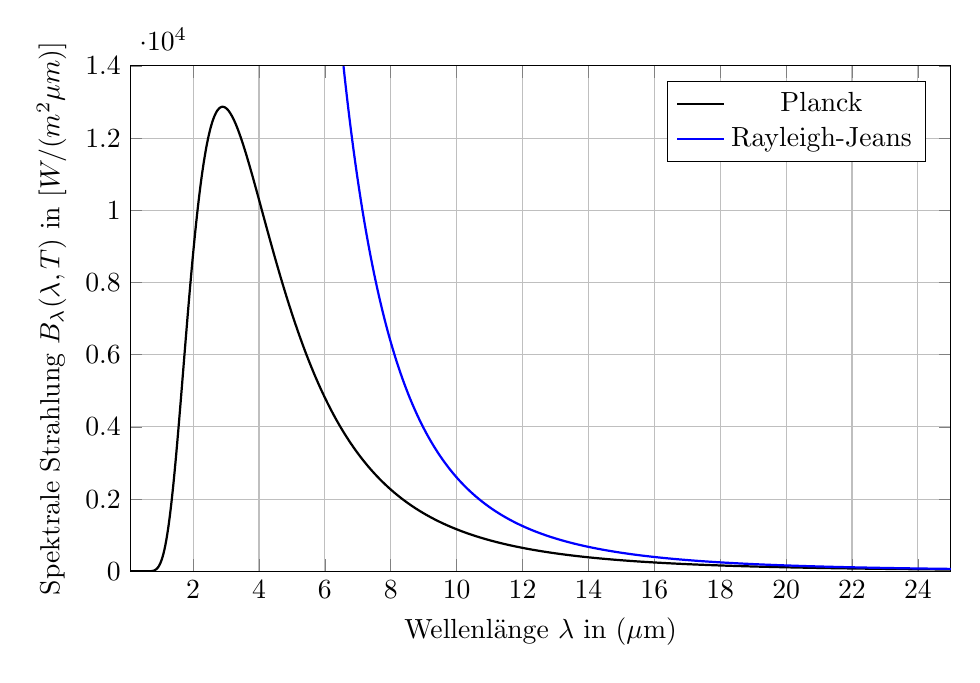
\begin{tikzpicture}
			
			% Hauptachse (linke y-Achse; Werte von 0 bis 14000)
			\begin{axis}[
				name=leftaxis,
				width=12cm,
				height=8cm,
				xlabel={Wellenlänge $\lambda$ in ($\mu$m)},
				ylabel={Spektrale Strahlung $B_\lambda(\lambda, T)$ in $[W/(m^2 \mu m)]$},
				xmin=0.1, xmax=25,
				ymin=0, ymax=14000,
				legend style={at={(0.97,0.97)}, anchor=north east},
				grid=both,
				domain=0.01:26,
				samples=1000
				]
				%W\,m$^{-2}$m$^{-1}
				% Konstanten (SI)
				\def\h{6.62607015e-34}       % Plancksche Konstante
				\def\c{2.99792458e8}         % Lichtgeschwindigkeit
				\def\kB{1.380649e-23}        % Boltzmann-Konstante
				\def\T{1000}                 % Temperatur in Kelvin
				
				% --- Plancksche Strahlungsformel ---
				\addplot[black, thick] 
				expression{
					(2*pi*\h*\c^2)/((x*1e-6)^5) * 1/(exp(\h*\c/((x*1e-6)*\kB*\T)) - 1) / 1e6
				};
				\addlegendentry{Planck}
				
				
				% --- Rayleigh-Jeans-Gesetz (Langwellennähe) ---
				\addplot[blue, thick, restrict y to domain=0:14000]
				expression{
					(2*pi*\c*\kB*\T)/((x*1e-6)^4) / 1e6
				};
				\addlegendentry{Rayleigh-Jeans}
				
				
			\end{axis}
			
			
			
		\end{tikzpicture}
		\caption{Strahlungsspektren nach Planck und Rayleigh-Jeans bei $T=1000\,\mathrm{K}$}
	\end{figure}
		

	In beiden Formeln kommen diverse Konstanten vor: Pi, die Bolzmann Konstante $k_B$, die Lichtgeschwindigkeit $c$ und $h$. 
	Er führte eine neue Naturkonstante ein, das Plancksche Wirkungsquantum $h = 6{,}626 \times 10^{-34} \ \text{J\,s}$. 
	Wie oben erwähnt entstand $h$ rein experimentell und war erst als mathematisches Trick gedacht. 
	
	
	Früher nahm man an, die Energie einer Welle hänge nur von ihrer Amplitude ab. 
	Man glaubte auch, Atome könnten jede beliebige Energiemenge abstrahlen. Plancks Modell stellte das infrage. 
	Nun konnte Energie nur in bestimmten Portionen abgegeben werden, abhängig von der Frequenz und nicht von der Amplitude.
	
	
	\begin{equation}
		E = h \cdot f
	\end{equation}
	 
	 
	Je höher die Frequenz, desto grösser ist das nötige Energiepaket. 
	Deshalb nimmt die Strahlung bei hohen Frequenzen wieder ab. 
	Denn hohe Frequenzen bedeuten viel Energie pro Lichtquant und es ist ziemlich unwahrscheinlich, dass ein einzelnes Atom so viel Energie auf einen Schlag abgibt. 
	Planck wusste dies nicht. 
	Aber mit dieser Formel war der erste Schritt in Richtung  Quantentheorie gemacht.
	
	%Einstein
	
	
	1905 kam Albert Einstein ins Spiel. 
	Er griff diese Formel auf, um den photoelektrischen Effekt zu erklären. 
	Er interpretierte sie so, dass Licht tatsächlich aus Teilchen (Photonen) besteht, die jeweils die Energie $E = h \cdot f$ tragen, also nicht nur als mathematischer Trick wie bei Planck, sondern als reale physikalische Aussage über die Natur des Lichts.
	Für diese Arbeit bekam er 1921 den Nobelpreis und nicht für seine Relativitätstheorie, wie viele denken.
	
	 
	%Bohr
	
	%Auskommentier, da exkurs (Atommodell)
	
	%1913 übertrug Niels Bohr die Quantisierung auf Atome. 
	%In seinem Modell befinden sich Elektronen in Schalen, dazuwischen ist nichts. 
	%Ein Übergang zwischen diesen diskreten Schalen ging immer mit einer Energieabgabe oder aufnahme in Form eines Photons einher. 
	%Auch wenn sein Modell längst überholt ist, war seine Idee von Schalen Grundlegend korrekt. 

	%de Broglie
	
	1924 stellte Louis de Broglie eine revolutionäre Idee vor.
	Nicht nur Licht besitzt Wellencharakter, auch Materie, also Teilchen wie Elektronen, könnten wellenartige Eigenschaften haben.
	Er vermutete, dass jedem Teilchen mit Impuls p eine Wellenlänge λ zugeordnet werden kann:
	
	\begin{equation}
		\lambda = \frac{h}{p}
	\end{equation}	
	
	Mit dieser einfachen Formel verband de Broglie die Vorstellung von Teilchen und Wellen. Damit wurde erstmals verständlich, warum sich auch Elektronen in bestimmten Experimenten wie Wellen verhalten.
	Kurios ist, dass jedes Objekt eine Wellenlänge hat, auch ein Fussball.
	Angenommen man schiesst ein Fussball mit der Masse von 0.45 $kg$ mit der Geschwindigkeit von 20 $m/s$.
	
	\begin{equation}
		\lambda = \frac{h}{p} = \frac{h}{m \cdot v} = 	\frac{6{,}626 \cdot 10^{-34} \ \text{Js}}{0{,}45 \ \text{kg} \cdot 20 \ \text{m/s}} \approx 7{,}36 \cdot 10^{-35} \ \text{m}
	\end{equation}	
	
	Die Berechnung zeigt, dass der Fussball eine extrem kleine Wellenlänge hat, somit besitzt er Wellencharakteristiken.
	Das Resultat ist absurd und hat in der Realität keinerlei bedeutung.
	Solche Rechnungen machen nur in der Quantenwelt Sinn, auch wenn die Gleichungen für alle Objekte gelten. 
	De Broglie zeigte, dass Wellen als Teilchen intepretiert werden können und umgekehrt. 
	
	
	
	%Schrödinger
	Erwin Schrödinger formulierte 1926 eine Gleichung, die das Verhalten von Teilchen als Wellen beschreibt. 
	Sie bildet die Grundlage der Quantenmechanik. Die Lösung dieser Gleichung ist die Wellenfunktion \( \psi(x, t) \). Sie liefert keine feste Bahn, sondern eine Wahrscheinlichkeitsverteilung für den Aufenthaltsort eines Teilchens.  
	Die eindimensionale zeitabhängige Schrödingergleichung lautet:
	
	\begin{equation}
		i \hbar \frac{\partial \psi(x,t)}{\partial t} = -\frac{\hbar^2}{2m} \frac{\partial^2 \psi(x,t)}{\partial x^2} + V(x) \psi(x,t)
	\end{equation}
	
	
	Um herauszufinden, wie wahrscheinlich ein Teilchen an einem Ort ist, muss man den Betrag von \( \psi(x, t) \) quadrieren. 
	Die resultierende Funktion \( |\psi(x, t)|^2 \) ist die Aufenthaltswahrscheinlichkeit. 
	Das Symbol \( \hbar \) steht für das reduzierte Plancksche Wirkungsquantum und ist gleich \( \frac{h}{2\pi} \). 
	
	Die Reise begann mit Plancks Energiepaketen, führte über Einsteins Lichtteilchen und de Broglies Materiewellen hin zu Schrödingers Wahrscheinlichkeitswellen. 
	Doch all diese Ideen behandelten Teilchen meist als isolierte Objekte.
	
	Die Quantenfeldtheorie geht einen Schritt weiter.
	Sie sagt, dass Teilchen gar nicht mehr als kleine Kügelchen existieren, sondern als Anregungen von Feldern, die den gesamten Raum durchdringen. 
	Elektronen, Photonen und alle anderen Teilchen sind Wellen in ihren jeweiligen Quantenfeldern.
	
	Damit verschmilzt die Teilchenwelt mit der Feldvorstellung.
	Nicht das Teilchen ist grundlegend, sondern das Feld und was wir beobachten, sind nur dessen kleinste Schwingungen.
	
	So wird aus der Quantenmechanik eine Feldtheorie.
	
\subsection{Der harmonische Oszillator\label{fourier:subsection:derHarmonischeOszillator}}
Warum genau schauen wir uns den harmonischen Oszillator an?
In der Quantenelektrodynamik werden die elektromagnetischen Felder als quantisierte harmonische Oszillatoren modelliert, deren Energie ebenfalls in Vielfachen von $\hbar\cdot\omega$ vorliegt.
Die Zustände des Feldes (Photonenzahlenzustände) werden durch die Schwingungszustände des harmonischen Oszillators beschrieben.

Diese Quantisierung erklärt, warum Licht in Lasern nicht kontinuierlich, sondern in diskreten Paketen (Photonen) emittiert wird. % todo: diesen Satz an anderer passenden Stelle einfügen

Die Wellengleichung lautet bekanntlich
\begin{equation}
    \frac{\partial^2 u}{\partial t^2} = c^2 \left( \frac{\partial^2 u}{\partial x^2} + \frac{\partial^2 u}{\partial y^2} \right).
\end{equation}
Wenn nun der y-Anteil als konstant betrachtet wird, sind alle partiellen Ableitungen nach y gleich Null.
Dies führt zu der vereinfachten Gleichung
\begin{equation}
    \frac{\partial^2 u}{\partial t^2} = c^2 \frac{\partial^2 u}{\partial x^2}.
\end{equation}
Daraus lässt sich die Differentialgleichung
\begin{equation}
    \ddot{a}(t) = -k^2 a(t)
\end{equation}
aufstellen.
$a(t)$ ist hierbei ein Fourier-Koeffizient des elektromagnetischen Wellenfeldes.
Die Lösung dieser Differentialgleichung lautet
\begin{equation}
    u(t,x) = a_k(t) \cos(kx)
\end{equation}

% Besser sin verwenden --> besser e^ikx verwenden; Überlegen, ob wir komplex arbeiten möchten
% In Präsentation mit cos und im Paper mit e^ikx


% Wichtiger Schritt: Der harmonische Oszillator in der Quantenmechanik --> Unterlagen anschauen. 
% Evtl. Termin mit ihm, um Unklarheiten zu klären.

% Gutes Video, welches den harmonischen Oszillator erklärt.
%       https://www.youtube.com/watch?v=5P19hROy9vk
% quantenmechanik: Energie ist auch Quantisiert;
% Oszillator kann nur auf bestimmten Leveln schwingen.
% Energielevel haben dieselben Abstände (quadratischer Brunnen)

% further theory: https://www.youtube.com/watch?v=OdizRUe84bg&list=PL8W2boV7eVfmdWs3CsaGfoITHURXvHOGm

Diese Gleichung ist analog zur Gleichung eines Federpendels.
Es handelt sich hier um ein ``Quanten-Federpendel''.    
\begin{figure}
\centering
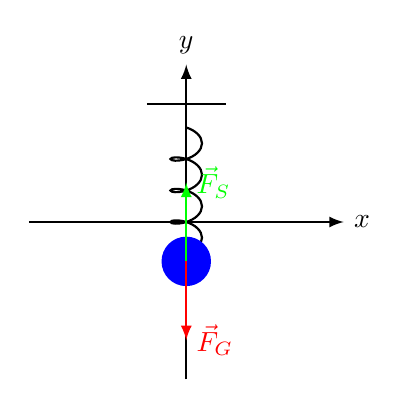
\begin{tikzpicture}[>=latex,thick]
    % Koordinatensystem
    \draw[->] (-2,0) -- (2,0) node[right] {$x$};
    \draw[->] (0,-2) -- (0,2) node[above] {$y$};
    
    % Feder
    \draw[thick] (0,1.5) -- (0,1.2);
    \draw[thick, decorate, decoration={coil, aspect=0.5, segment length=4mm, amplitude=2mm}] (0,1.2) -- (0,-0.5);
    
    % Körper
    \filldraw[blue] (0,-0.5) circle (0.3) node[below] {$m$};
    
    % Kräfte
    \draw[->, thick, red] (0,-0.5) -- (0,-1.5) node[right] {$\vec{F}_G$};
    \draw[->, thick, green] (0,-0.5) -- (0,0.5) node[right] {$\vec{F}_S$};
    
    % Aufhängung
    \draw[thick] (-0.5,1.5) -- (0.5,1.5);
\end{tikzpicture}
\caption{Federpendel}\label{fourier:figure:federpendel}
\end{figure}

%%
\subsection{Einführung in Werkzeuge der Quantenmechanik\label{fourier:subsection:werkzeugeQuantenmechanik}}
Für die Erklärung von Photonen sind einige Werkzeuge der Quantenmechanik nützlich, welche nachfolgend kurz eingeführt werden.

\subsubsection{Bra-Ket-Notation\label{fourier:subsubsection:braKetNotation}} % todo knma: dies verständlicher formulieren und, dass man das dann als Werkzeug gebrauchen kann, um Photon zu beweisen
Die Bra-Ket-Notation, auch Dirac-Notation genannt, wurde von Paul Dirac eingeführt und ist heute Standard in der Quantenmechanik.
Sie dient dazu, Zustände und Operatoren kompakt und elegant darzustellen.

Ein \emph{Ket} $|\psi\rangle$ beschreibt den Zustand eines quantenmechanischen Systems.
Man kann sich Kets wie Richtungs-Pfeile vorstellen, die angeben, ``wie'' das System gerade ist;
z.B. mit welcher Energie, welchem Spin oder an welchem Ort sich ein Teilchen befindet.
Ein \emph{Bra} $\langle\psi|$ ist das zugehörige Gegenstück zum Ket.
Es steht symbolisch für eine Messung oder einen Test auf diesen Zustand.
Formal ist es das komplex-konjugierte und transponierte Objekt zum Ket.

Beispiele:
\begin{itemize}
  \item $|0\rangle$ kann den Grundzustand eines Systems beschreiben.
  \item $|x\rangle$ steht für einen Zustand, in dem sich ein Teilchen genau am Ort $x$ befindet.
  \item Allgemeine Zustände lassen sich als Superposition (Überlagerung) schreiben, z.B.:
  \[
    |\psi\rangle = \alpha\,|0\rangle + \beta\,|1\rangle,
  \]
  wobei $\alpha$ und $\beta$ komplexe Zahlen sind.
\end{itemize}

Das \emph{Skalarprodukt}
\begin{equation}
  \langle \phi | \psi \rangle = \int\limits_{-\infty}^{+\infty} \phi^*(x)\,\psi(x)\,dx,
\end{equation}
ist eine einzige (meist komplexe) Zahl, die angibt, wie ``gleich'' oder ``verschieden'' sich die beiden Zustände $|\phi\rangle$ und $|\psi\rangle$ verhalten.
Man multipliziert dafür $\phi^*(x)$ (das konjugiert-komplexe von $\phi$) mit $\psi(x)$ und integriert über den gesamten Raum.
\begin{itemize}
	\item Liegen die Zustände genau übereinander, erhält man den Betrag 1 (bei Normierung).
	\item Sind sie orthogonal, also völlig verschieden, ist das Ergebnis 0.
\end{itemize}
Kurz gesagt:
$\langle \phi | \psi \rangle$ misst die Überlappung (den ``Winkel'') zwischen zwei Quantenzuständen.

Die \emph{Norm} eines Zustands ist einfach das Skalarprodukt mit sich selbst:
\begin{equation}
  \langle \psi | \psi \rangle = \int \psi^*(x)\,\psi(x)\,dx.
\end{equation}

Der \emph{Erwartungswert} eines physikalischen Operators $A$ im Zustand $|\psi\rangle$ beschreibt den durchschnittlich gemessenen Wert bei vielen Wiederholungen:
\begin{equation}
  \langle A \rangle = \langle \psi | A | \psi \rangle = \int \psi^*(x)\,(A\psi)(x)\,dx.
\end{equation}

Ist $|\psi\rangle$ ein Eigenzustand von $A$ mit einem bestimmten Eigenwert $a$, d.h.
\begin{equation}
  A\,|\psi\rangle = a\,|\psi\rangle,
\end{equation}
so ergibt eine ideale Messung des Operators $A$ immer genau den Wert $a$.

Die Bra-Ket-Notation ist nicht nur kompakt, sondern macht viele Rechnungen in der Quantenmechanik übersichtlich und leicht handhabbar.

\subsubsection{Heisenbergs Unschärferelation%
\label{fourier:subsubsection:unschaerferelation}}
In der Quantenmechanik gibt es keine festen Werte für Grössen wie Ort oder Impuls eines Teilchens, sondern nur Wahrscheinlichkeiten und Mittelwerte, wo sich diese befinden oder wie schnell sie sind.
Im Gegensatz zur klassischen Physik, wo der Impuls $p$ eine klar definierte Zahl ist, wird in der Quantenmechanik der Impuls durch einen sogenannten Operator beschrieben:
\begin{equation}
	\hat{p} = \frac{\hbar}{\mathrm{i}} \frac{d}{dx}.
\end{equation}
Das bedeutet:
Man kann nicht einfach sagen ``Das Teilchen hat genau diesen Impuls'', sondern der Impuls ist grundsätzlich unscharf (nicht exakt bestimmbar).
Ort und Impuls sind sogenannte nicht gleichzeitig messbare Grössen:
Ihre Operatoren ``vertauschen'' nicht miteinander, was mathematisch ausgedrückt wird durch
\begin{equation}
	[\hat{x},\hat{p}] = \hat{x} \hat{p} - \hat{p} \hat{x} = \mathrm{i} \hbar.
\end{equation}
Diese fehlende Vertauschbarkeit führt direkt zur bekannten Unschärferelation.
Ihre Herleitung basiert auf einer grundlegenden mathematischen Ungleichung, der sogenannten Cauchy-Schwarz-Ungleichung:
\begin{equation}
	\vec{a} \bullet \vec{b} = |\vec{a}| |\vec{b}|\cos\alpha \le |\vec{a}| |\vec{b}|.
\end{equation}
die besagt, dass das Skalarprodukt zweier Vektoren nie grösser sein kann als das Produkt ihrer Längen.
Übertragen auf die Wellenfunktionen zweier Quantenzustände $|\phi\rangle$ und $|\chi\rangle$, erhält man
\begin{equation}
	|\langle\phi | \chi\rangle|^2 \le \langle\phi | \phi\rangle \langle\chi | \chi\rangle.
\end{equation}
Diese Relation stellt eine fundamentale Schranke für das Skalarprodukt zweier Zustände dar.
Der Ausdruck $|\langle\phi|\chi\rangle|^2$ misst die Überlappung der beiden Zustände, also gewissermaßen, wie ähnlich sie sich sind.
Die Terme $\langle\phi|\phi\rangle$ und $\langle\chi|\chi\rangle$ entsprechen dabei den Quadraten der Längen (Normen) der Zustände.
Der Betrag des Skalarprodukts kann also niemals größer werden als das Produkt der Normen, ganz analog zur klassischen Vektoranalysis.
Das Quadrat auf der linken Seite ergibt sich, weil die Ungleichung eine Aussage über den Betrag des Skalarprodukts ist, während die rechte Seite stets reell und positiv ist.
Diese Form der Ungleichung bildet die mathematische Grundlage für die Herleitung der Heisenbergschen Unschärferelation.
Die Zustände $|\phi\rangle$ und $|\chi\rangle$ sind hier in der sogenannten Bra-Ket-Notation geschrieben, einer kompakten Notation für Zustände in der Quantenmechanik, wie sie in Abschnitt~\ref{fourier:subsubsection:braKetNotation} eingeführt wurde.

Setzt man
\begin{equation}
	|\phi\rangle = (\hat{x} - \langle \hat{x} \rangle) |\psi\rangle \quad |\chi\rangle = (\hat{p} - \langle \hat{p} \rangle) | \psi\rangle,
\end{equation}
also die Abweichungen von Ort und Impuls gegenüber ihren Mittelwerten ein, so führen die Definitionen
\begin{equation}
	\sigma_x^2 = \langle\phi | \phi\rangle \quad \sigma_p^2 = \langle\chi | \chi\rangle
\end{equation}
für die sogenannten Standardabweichungen --ein Mass für die „Streuung“ oder Unschärfe-- zusammen mit
\begin{equation}
	\langle\psi | [\hat{x},\hat{p}] | \psi\rangle = \mathrm{i}\hbar
\end{equation}
zur Beziehung:
\begin{equation}
	\sigma_x^2 \sigma_p^2 \ge \frac{1}{4} |\langle\psi | [\hat{x},\hat{p}] | \psi\rangle|^2 = \frac{\hbar^2}{4},
\end{equation}
und damit schliesslich zur bekannten Form der Unschärferelation:
\begin{equation}
	\sigma_x \sigma_p \ge \frac{\hbar}{2}.
\end{equation}

Hier bedeuten $\sigma_x$ und $\sigma_p$ die Unschärfen (Standardabweichungen) in Ort und Impuls.
Die Unschärferelation sagt also:
Je genauer der Ort eines Teilchens bekannt ist (kleines $\sigma_x$), desto unschärfer muss sein Impuls ($\sigma_p$) sein --und umgekehrt.
Das zeigt anschaulich die Wellennatur von Teilchen:
Ein Teilchen, das genau lokalisiert ist, muss eine breite Wellenverteilung im Impulsraum haben.
Würde man das $\tfrac{1}{2}$ in der Formel weglassen, erhielte man eine vereinfachte, aber weniger präzise Darstellung des Zusammenhangs.
%%%%%%%%%%%%%%%%%%%%%%%%%%%%%%%%
% todo knma: Ergänzungen anbringen

\subsection{Beweis des Photons\label{fourier:subsection:beweisPhoton}}
In diesem Abschnitt verwenden wir die bisher eingeführten Grundlagen der Quantenmechanik, um zu zeigen, dass Licht nicht kontinuierlich, sondern in kleinsten Energiepaketen, sogenannten Photonen, übertragen wird.

Wir starten mit der klassischen Hamilton-Funktion, die die Gesamtenergie eines Systems beschreibt:
\begin{equation}
	H(x, p) = T(p) + V(x),
\end{equation}
wo $T(p)$ die kinetische Energie und $V(x)$ die potenzielle Energie des Teilchens darstellen.

%%% maybe todo: add some stuff of book quantum mechanics to glue things together

Durch Schrödinger wird der Impuls p durch
\begin{equation}
	\frac{\hbar}{\mathrm{i}} \frac{\partial}{\partial x}
\end{equation}
ersetzt.
Wodurch der Hamiltonoperator
\begin{equation}
	\hat{H} = -\frac{\hbar^2}{2m}\frac{\partial^2}{\partial x^2} + V(x)
\end{equation}	
resultiert.

Der Erwartungswert des Impulses in einem Zustand $|\psi\rangle$ lässt sich schreiben als:
\begin{equation}
	E(p) = \int \bar{\psi}p\psi dx
	= \int \bar{\psi} \frac{\hbar}{i} \frac{d\psi}{dx} dx
	= \langle \psi | p | \psi \rangle
\end{equation}
Er gibt an, welcher mittlere Impuls gemessen wird, wenn sich das System im Zustand $|\psi\rangle$ befindet.

Nach Heisenbergs Unschärferelation (siehe Abschnitt~\ref{fourier:subsubsection:unschaerferelation}) gilt in der Quantenmechanik, dass die Vertauschung der Impuls- und Ortsoperatoren nicht null ist, also
\begin{equation}
	px \neq xp.
\end{equation}
Die Vertauschungsrelation kann als
\begin{equation}
	[x, p] = \hbar id
\end{equation}
geschrieben werden.


%%%%%%%%%%%%%%%%%%%%% dieser Abschnitt nötig/ an anderem Ort einfügen
% todo knma: Abschnitt evtl. weg oder an anderem Ort? War in seinen Notizen.
\begin{equation}
	\vec{a}\bullet\vec{b} = |\vec{a}| \cdot |\vec{b}| \cdot \cos{\alpha} \leq |\vec{a}| \cdot |\vec{b}|
\end{equation}
% todo: some text
\begin{equation}
	\int \langle \psi |xp|\psi \rangle\,dx	% todo: Was soll uns diese Gleichung sagen?
\end{equation}
% todo: some text
%%%%%%%%%%%%%%%%%%%%%%%%%%%

Um nun den Beweis für das Photon zu führen, betrachten wir den harmonischen Oszillator (Abschnitt~\ref{fourier:subsection:derHarmonischeOszillator}).
Hierfür führen wir dimensionslose Operatoren ein:
\[ 
Q = \sqrt{\frac{m\omega}{\hbar}}x
\qquad\text{und}\qquad
P = \frac{1}{\sqrt{m\hbar\omega}}p.
\]
Der Hamilton-Operator nimmt dann die Form an:
\begin{equation}
	H = \frac{1}{2}(P^2 + Q^2).
\end{equation}

Nun definieren wir die sogenannten Leiteroperatoren:
\[
a^{+} = \frac{1}{\sqrt{2}}(Q + iP)
\qquad\text{und}\qquad
a = \frac{1}{\sqrt{2}}(Q - iP).
\]

%% todo: here knma
Mit der Vertauschungsrelation
\begin{equation}
	[P,Q] = -\mathrm{i} \cdot id,
\end{equation}
wobei id die Einheitsmatrix ist, lässt sich über den Hamiltonoperator % todo: ist es wirklich der und Satz vervollstängigen
%todo blablabla
\begin{equation}
	H = \frac{1}{2}(P^2+Q^2)
\end{equation}
\begin{equation}
	H - \frac{1}{2} = N
\end{equation}
\begin{equation}
	\textcolor{blue}{[a, a^+] = 1}
\end{equation}
\begin{equation}
	N = a^+a + \frac{1}{2}
\end{equation}
\begin{equation}
	N\cdot a^+ - a^+N 
	= \textcolor{blue}{a^+a}a^+ + \cancel{\frac{1}{2}a^+} \textcolor{blue}{-a^+a}a^+ - \cancel{\frac{1}{2}a^+}
	= a^+\textcolor{blue}{[a, a^+]}
	= \textcolor{blue}{1}\cdot a^+
\end{equation}
% todo: tbc

%%%%%%%%%%%%%%%%%%%%%%%%%%%%%%%%%%%%%%%%%%%%%%%%%%%%%%%%%%%%%%%%%%%%%%%%%%%%%%%%%%%%%%%%%%%%%%

% Quantisierung vom Feld --> Erklärung Photon, Schwierigkeit von Polarisation erwähnen, E und B

% Für jede Wellenlänge gibt es einen Fourier-Koeffizienten, davon kommen die a's

-----------------------------------------------------------------------------------

% todo: Diese Gleichung mit Erklärungen irgendwo einflechten.
% question: Wo wäre es sinnvoll?
Mit dem Hamiltonoperator in der Form
\begin{equation}
	H = \hbar\omega(N + \frac{1}{2})
\end{equation}
folgt die Eigenwertgleichung
\begin{equation}
	H\,|\psi_n\rangle = E_n\,|\psi_n\rangle,
  	\quad
	E_n = \hbar\omega\Bigl(n + \tfrac12\Bigr).
\end{equation}
Dabei ist $n = 0,1,2,\dots$ die Besetzungszahl (Photonenzahl beim Lichtfeld).
Das zeigt, dass $|\psi_n\rangle$ die stationären Energiezustände sind und die Energiewerte quantisiert in Schritten von $\hbar\omega$ liegen.

% todo: diese Formeln genauer ausführen und in Kapitel einbinden.
\begin{equation}
	a^+ |\psi_n\rangle \rightarrow a^+ | \psi_n\rangle
\end{equation}
Energie
\begin{equation}
	H(a^+ | \psi_n\rangle) = ...
	= (1 + \epsilon_n) a^+ | \psi_n\rangle % todo ausführen
\end{equation}
$(1+\epsilon_n)$ = EW = Energie % todo: direkt darunter
\begin{equation}
	a^- |\psi_n\rangle \rightarrow a^-|\psi_n\rangle
\end{equation}
\begin{equation}
	H(a^-|\psi_n\rangle) = ...
	= (-1 + \epsilon_n) a^- |\psi_n\rangle % todo: ausführen
\end{equation}

Final text % todo: this is only a filler
